% v2-acmsmall-sample.tex, dated March 6 2012
% This is a sample file for ACM small trim journals
%
% Compilation using 'acmsmall.cls' - version 1.3 (March 2012), Aptara Inc.
% (c) 2010 Association for Computing Machinery (ACM)
%
% Questions/Suggestions/Feedback should be addressed to => "acmtexsupport@aptaracorp.com".
% Users can also go through the FAQs available on the journal's submission webpage.
%
% Steps to compile: latex, bibtex, latex latex
%
% For tracking purposes => this is v1.3 - March 2012

\documentclass[prodmode,acmtecs]{acmsmall} % Aptara syntax

\usepackage{graphicx}
\usepackage{caption}
\usepackage{subfigure}
\usepackage{setspace}
\usepackage{tabulary}
\newcommand{\specialcell}[2][c]{%
  \begin{tabular}[#1]{@{}c@{}}#2\end{tabular}}

\usepackage{lineno}
\usepackage{xfrac}


\usepackage{alltt}
\renewcommand{\ttdefault}{txtt}

\usepackage{listings}
\lstset{language=C, breaklines=true}

\usepackage[cmex10]{amsmath}
\usepackage{url}

% Package to generate and customize Algorithm as per ACM style
\usepackage[ruled]{algorithm2e}
\renewcommand{\algorithmcfname}{ALGORITHM}
\SetAlFnt{\small}
\SetAlCapFnt{\small}
\SetAlCapNameFnt{\small}
\SetAlCapHSkip{0pt}
\IncMargin{-\parindent}

% Metadata Information
%\acmVolume{9}
%\acmNumber{4}
%\acmArticle{39}
%\acmYear{2010}
%\acmMonth{3}

% Document starts
\begin{document}

% Page heads
\markboth{F. Luporini et al.}{Optimizing Automated Finite Element Integration through Expression Rewriting and Code Specialization}

% Title portion
\title{Optimizing Automated Finite Element Integration through Expression Rewriting and Code Specialization}
\author{Fabio Luporini
\affil{Imperial College London}
David A. Ham
\affil{Imperial College London}
Paul H.J. Kelly
\affil{Imperial College London}}

\begin{abstract}
Abstract goes here
%
%The code is generated from a high level language for PDEs. An
%invocation of the kernel typically does tensor-like calculators over
%relatively small matrices; e.g., triply nested loops operating on
%about a dozen iterations. Because of the DSL context, COFFEE has a lot
%of flexibility on how it organizes/orders the calculations to tailor
%execution to a target architecture.
%
\end{abstract}

\category{G.1.8}{Numerical Analysis}{Partial Differential Equations -
  Finite element methods}

\category{G.4}{Mathematical Software}{Parallel and vector
  implementations}

\terms{Design, Performance}

\keywords{Finite element integration, local assembly, compilers,
  optimizations, SIMD vectorization}

\acmformat{Fabio Luporini, David A. Ham, and Paul   H. J. Kelly, 2014. 
  Optimizing Automated Finite Element Integration through Expression Rewriting and Code Specialization.}

% At a minimum you need to supply the author names, year and a title.
% IMPORTANT: Full first names whenever they are known, surname last,
% followed by a period.  In the case of two authors, 'and' is placed
% between them.  In the case of three or more authors, the serial
% comma is used, that is, all author names except the last one but
% including the penultimate author's name are followed by a comma, and
% then 'and' is placed before the final author's name.  If only first
% and middle initials are known, then each initial is followed by a
% period and they are separated by a space.  The remaining information
% (journal title, volume, article number, date, etc.) is
% 'auto-generated'.

\begin{bottomstuff}

This research is partly funded by the MAPDES project, by the
Department of Computing at Imperial College London, by EPSRC through
grants EP/I00677X/1, EP/I006761/1, and EP/L000407/1, by NERC grants
NE/K008951/1 and NE/K006789/1, by the U.S.  National Science
Foundation through grants 0811457 and 0926687, by the U.S. Army
through contract W911NF-10-1-000, and by a HiPEAC collaboration
grant. The authors would like to thank Dr. Carlo Bertolli,
Dr. Lawrence Mitchell, and Dr. Francis Russell for their invaluable
suggestions and their contribution to the Firedrake project.

Author's addresses: Fabio Luporini $\&$ Paul H. J. Kelly, Department of Computing,
Imperial College London; David A. Ham, Department of Computing and
Department of Mathematics, Imperial College London; 
\end{bottomstuff}

\maketitle

%Computational cost is a critical limitation in scientific computing,
%especially for finite element simulations. To provide one particular
%example we are particularly concerned about, it has been well
%established that mesh resolution Consequently, our aggressive
%optimization of local assembly, which may even take up to 60% of the
%overall FEM's execution time, directly impacts the performance of
%large-scale scientific simulations running on supercomputers.

\section{Introduction}

The need for rapidly implementing high performance, robust, and portable finite element methods has led to approaches based on automated code generation. This has been proved successful in the context of the FEniCS~\cite{Fenics} and Firedrake~\cite{firedrake-code} projects, which have become incredibly popular over the last years. In these frameworks, the weak variational form of a given problem is expressed at high-level by means of a domain-specific language. Such a mathematical specification is suitably manipulated and then passed as input to a form compiler, whose goal is to generate a representation of local assembly operations. These operations numerically evaluate problem-specific integrals in order to compute so called local matrices and vectors, which represent the contributions from each element in the discretized domain to the equation solution. Local assembly code must be high performance: as the complexity of a variational form increases, in terms of number of derivatives, pre-multiplying functions, and polynomial order of the chosen function spaces, the resulting assembly kernels become more and more computationally expensive, covering a significant fraction of the overall computation run-time. 

Achieving high performance implementations is, however, non-trivial. The complexity of mathematical expressions involved in the numerical integration, which varies from problem to problem, and the small size of the loop nest in which such integral is computed obstruct the optimization process. Also, traditional vendor compilers, such as \emph{GNU's} and \emph{Intel's}, fail at exploiting the structure inherent assembly expressions. This has led to development of a number of higher-level approaches to optimize local assembly kernels.  In~\cite{quadrature1}, it is shown how automated code generation can be leveraged to introduce domain-specific optimizations, which a user cannot be expected to write ``by hand''. \cite{Kirby-FEM-opt} and~\cite{Francis} have studied, instead, different optimization techniques based on a mathematical reformulation of the problem. In~\cite{Luporini}, we have made one step forward by showing that different problems, on different platforms, require distinct set of transformations if close-to-peak performance needs to be obtained, and that low-level, domain-aware code transformations are essential to maximize instruction-level parallelism and register locality. The problem of optimizing local assembly routines has been tackled recently also for GPUs, for instance in~\cite{petsc-integration-gpu},~\cite{Klockner}, and~\cite{Bana}.

Our research has resulted in the development of a compiler, COFFEE\footnote{COFFEE stands for COmpiler For FinitE Element local assembly.}, fully integrated with the Firedrake framework. While clearly separating the mathematical domain, which remains captured in the higher-level form compiler, from the optimization process, COFFEE also aims to be platform-agnostic. The code transformations occur on an intermediate representation of the assembly code, which is ultimately translated into platform-specific code. Domain knowledge is exploited in two ways: for simplifying the implementation of a broad range of code transformations, and, obviously, to make them extremely effective. Domain knowledge is conveyed to COFFEE from the higher level (the form compiler in the case of Firedrake, although any user-provided code would be acceptable) through suitable annotations attached to the input. For example, when the input is in the form of an abstract syntax tree produced by the form compiler, specific nodes are decorated so as to drive the optimization process. Although COFFEE has been thought of as a multi-platform optimizing compiler, our performance evaluation so far has been restricted to standard CPU platforms only. We emphasize once more, however, that the transformations applicable by both the Expression Rewriter (Section~\ref{sec:expr-rewriting}) and the Code Specializer (Section~\ref{sec:code-spec}) would work on generic accelerators as well.

In this paper, we build on the work presented in~\cite{Luporini} and present a novel structured approach to the optimization of automatically-generated finite element integration routines based on quadrature representation. We argue that peak performance can be achieved only by passing through a two-step optimization procedure: 1) expression rewriting, to minimize floating point operations, 2) and code specialization, to obtain, for instance, effective register utilization and SIMD vectorization. The code transformations introduced in~\cite{Luporini} are reused: as explained in Section~\ref{sec:summary-opts}, padding and data alignment, expression splitting, and vector-register tiling become sub-steps of code specialization; on the other hand, generalized loop-invariant code motion is a step of the expression rewriting process. More importantly, we complement and generalize our previous work with the following contributions.

Expression rewriting is based on a formal set of rewrite rules. Our first contribution consists of a framework that aggressively exploits associativity, distributivity, and commutativity of arithmetic operators to expose ``hidden'' loop-invariant sub-expressions. Secondly, we show how to make use of domain knowledge to avoid computation over zero-valued regions in vector-valued basis functions arrays, while preserving code vectorizability. These transformations will allow outperforming the results obtained in~\cite{Luporini} as well as those achievable by using FEniCS' built-in optimizations, presented in~\cite{quadrature1}. 

At code specialization time, transformations are applied to maximize the exploitation of the underlying platform's resources, e.g. SIMD lanes. On top of the work in~\cite{Luporini}, we provide a number of contributions. Firstly, we show the benefit of vector-expansion to achieve SIMD vectorization of otherwise scalar code. This is particularly useful in complex forms, like those based on hyperelasticity. Secondly, we answer an open problem in~\cite{Luporini} by providing an algorithm that automatically transforms an element matrix evaluation into a sequence of calls to BLAS' dense matrix multiplies. BLAS routines are known to perform far from peak performance when the involved arrays are small, which is almost always the case of low-order finite element methods. However, we will show that in corner, yet important cases, especially in forms characterized by pre-multiplying functions and relatively high-order function spaces, a BLAS-based execution strategy can be a successful. Finally, we introduce a model-driven, dynamic autotuner that automatically and transparently compose the set of code transformations that are likely to maximize the performance of a given problem. The main challenge with the autotuner is to maintain, for any possible problem, the search space reasonably small, although comprising the most effective code variants, so that the overhead, which impacts the run-time, is negligible. 

Expression rewriting and code specialization have been implemented in COFFEE and are fully operating. Therefore, to testify the goodness of our approach, we provide an extensive and unprecedented performance evaluation in a number of forms of increasing complexity, including problems based on hyperelasticity operators. We characterize our problems by varying polynomial order of the employed function spaces and number of pre-multiplying functions. To clearly distinguish the improvement achieved by this work, we will compare four sets of code variants, for each problem instance: 1) unoptimized code, i.e. a local assembly routine as returned from the form compiler; 2) code optimized by FEniCS, i.e. the work in~\cite{quadrature1}; 3) code optimized as described in~\cite{Luporini}; code optimized by expression rewriting and code specialization as described in this paper. Notable performance improvements of 4) over 1), 2) and 3) are reported and detailed.


%The contributions of this paper can be summarized as follows:
%\begin{enumerate}
%\item 
%\item extensive and unprecedented performance evaluation in a wide range of forms of increasing complexity
%\end{enumerate}

%Extensive performance evaluation...

%This paper can be thought of as a continuation of the work presented in~\cite{Luporini}: in particular, we answer the remaining open questions, generalize and formalize an approach to minimize redundant computation using a similar philosophy, we show ~\cite{quadrature1}. 

\section{Preliminaries}
\label{sec:background}

%is the computation of contributions of a specific cell in the discretized domain to the linear system which yields the PDE solution. The process consists of numerically evaluating problem-specific integrals to produce a matrix and a vector [Olgaard and Wells 2010; AMCG 2010], whose sizes depend on the order of the method. This operation is applied to all cells in the discretized domain. In this work we focus on local matrices, or “element matrices”, which are more costly to compute than element vectors.

\subsection{Quadrature for Finite Element Local Assembly}
We summarize the basic concepts sustaining the finite element method following the notation adopted in~\cite{quadrature1} and~\cite{Francis}. We consider the weak formulation of a linear variational problem
\begin{equation}
\begin{split}
Find\ u\ \in U\ such\ that \\
a(u, v) = L(v), \forall v \in V
\end{split}
\end{equation}
where $a$ and $L$ are called bilinear and linear form, respectively. The set of \textit{trial} functions $U$ and the set of \textit{test} functions $V$ are discrete function spaces. For simplicity, we assume $U = V$ and $\lbrace \phi_i \rbrace$ be the set of basis functions spanning $U$. The unknown solution $u$ can be approximated as a linear combination of the basis functions $\lbrace \phi_i \rbrace$. From the solution of the following linear system it is possible to determine a set of coefficients to express $u$
\begin{equation}
A\textbf{u} = b
\end{equation}
in which $A$ and $b$ discretize $a$ and $L$ respectively:
\begin{equation}
\centering
\begin{split}
A_{ij} = a(\phi_i(x), \phi_j(x)) \\
b_i = L(\phi_i(x))
\end{split}
\end{equation}
The matrix $A$ and the vector $b$ are computed in the so called assembly phase. Then, in a subsequent phase, the linear system is solved, usually by means of an iterative method, and $\textbf{u}$ is eventually evaluated. 

We focus on the assembly phase, which is often characterized as a two-step procedure: \textit{local} and \textit{global} assembly. Local assembly is the subject of the paper: this is about computing the contributions that an element in the discretized domain provide to the approximated solution of the equation. Global assembly, on the other hand, is the process of suitably ``inserting'' such contributions in $A$ and $b$. 

Without loss of generality, we illustrate local assembly in a real example, the evaluation of the local assembly (or, equivalently, element) matrix for a Laplacian operator. Consider the weighted Laplace equation
\begin{equation}
- \nabla \cdot (w \nabla u) = 0
\end{equation}
in which $u$ is unknown, while $w$ is prescribed. The bilinear form associated with the weak variational form of the equation is:
\begin{equation}
a(v, u) = \int_\Omega w \nabla v \cdot \nabla u\ \mathrm{d}x
\end{equation}
The domain $\Omega$ of the equation is partitioned into a set of cells (elements) $T$ such that $\bigcup T = \Omega$ and $\bigcap T = \emptyset$. By defining $\lbrace \phi_i^K \rbrace$ as the set of local basis functions spanning $U$ on the element $K$, we can express the local element matrix as
\begin{equation}
\label{stiffness}
A_{ij}^K = \int_K w \nabla \phi_i^K \cdot \nabla \phi_j^K\ \mathrm{d}x
\end{equation}
The local element vector $L$ can be determined in an analogous way. 
%From the computational perspective, its evaluation is however less expensive than that of $A$.

Quadrature schemes are conveniently used to numerically evaluate $A_{ij}^K$. For convenience, a reference element $K_0$ and an affine mapping $F_K : K_0 \rightarrow K$ to any element $K \in T$ are introduced. This implies a change of variables from reference coordinates $X_0$ to real coordinates $x = F_K (X_0)$ is necessary any time a new element is evaluated. The numerical integration routine based on quadrature representation over an element $K$ can be expressed as follows
\begin{equation}
\label{quadrature}
\scriptsize
A_{ij}^K = \sum_{q=1}^N \sum_{\alpha_3=1}^n \phi_{\alpha_3}(X^q)w_{\alpha_3} \sum_{\alpha_1=1}^d \sum_{\alpha_2=1}^d \sum_{\beta=1}^d \frac{\partial X_{\alpha_1}}{\partial x_{\beta}} \frac{\partial \phi_i^K(X^q)}{\partial X_{\alpha_1}} \frac{\partial X_{\alpha_2}}{\partial x_{\beta}} \frac{\partial \phi_j^K(X^q)}{\partial X_{\alpha_2}} det F_K' W^q
\end{equation}
where $N$ is the number of integration points, $W^q$ the quadrature weight at the integration point $X^q$, $d$ is the dimension of $\Omega$, $n$ the number of degrees of freedom associated to the local basis functions, and $det$ the determinant of the Jacobian matrix used for the aforementioned change of coordinates.  

In the next sections, we will often refer to the (local) element matrix evaluation, such as Equation~\ref{quadrature} for the weighted Lapalce operator, as the \textit{assembly expression} of the variational problem.


\subsection{COFFEE: a Compiler for Optimizing Quadrature-based Finite Element Integration}
\label{sec:summary-opts}
If high performance code needs to be generated, assembly expressions must be optimized with regards to three interrelated aspects: 1) arithmetic intensity, 2) instruction-level parallelism, and 3) data locality. In this paper, we tackle these three points building on our previous work (\cite{Luporini}).

\begin{figure}
\begin{center}
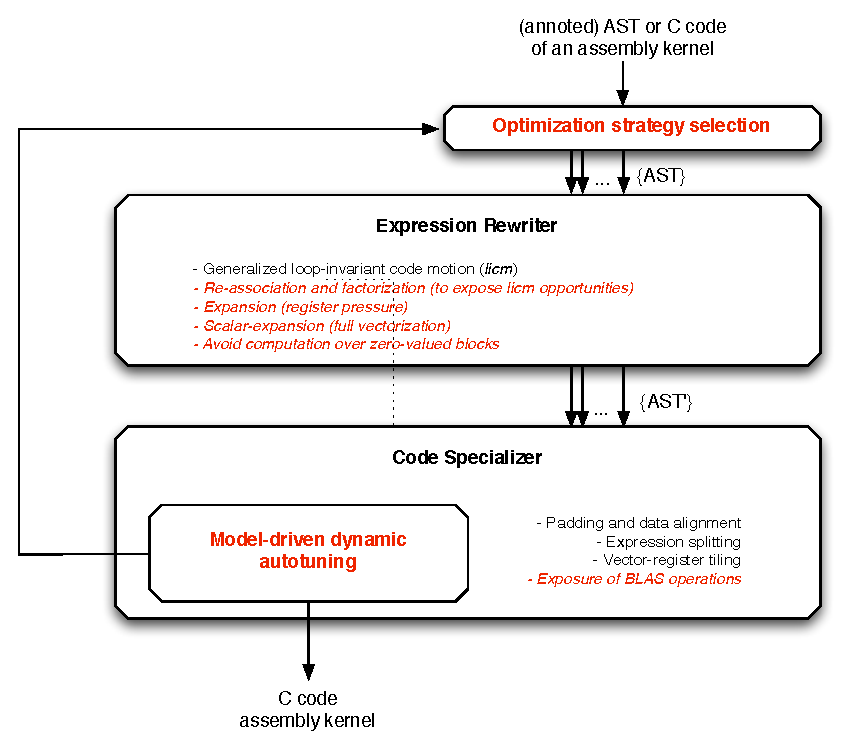
\includegraphics[scale=0.6]{pictures/coffee-scheme}
\caption{Outline of COFFEE}\label{fig:coffee-outline}
\end{center}
\end{figure}

COFFEE is a mature, platform-independent compiler capable of optimizing local assembly code. Its high-level structure can be outlined as in Figure~\ref{fig:coffee-outline}. The input is either suitably-annoted C code, explicitly provided by the user, or a decorated abstract syntax tree (henceforth AST) representation of an assembly kernel, automatically generated by the higher level in the stack. We have integrated COFFEE with the Firedrake framework; here, the input to COFFEE is originated by the FEniCS Form Compiler in the form of an AST. Decoration of special AST nodes, or equivalently annotation of C code, is extensively used to convey domain knowledge to COFFEE. This is used to introduce more effective, specialized optimizations, as well as to simplify implementation.

Two conceptually distinct software modules can be individuated: the Expression Rewriter and the Code Specializer. The former targets arithmetic intensity. Its role is to transform the assembly expression and, therefore, the enclosing loop nest, so as to minimize the number of floating point operations that are performed to evaluate the element matrix (or vector). The latter is tailored to optimizing for instruction-level parallelism, particularly SIMD vectorization, and data (register) locality. The Expression Rewriter manipulates and transforms the original AST, which is then provided to the Code Specializer. As described later, we have invested some effort to ensure that the code transformations applied in the expression rewriting stage do not break any code specialization opportunity. This for example would not be the case if the Expression Rewriter coincided with the FEniCS Form Compiler's built-in optimization system; we will clarify this aspect in Section~\ref{sec:zeros}.

To neatly distinguish the contributions of this paper from those in~\cite{Luporini}, in this section we summarize the results of our previous work. Moreover, in Section~\ref{sec:perf-results}, we will explicitly compare the performance achieved with the transformations presented in this paper to~\cite{Luporini} (as well as to FEniCS' built-in optimizations).

In our previous work, we have demonstrated the effectiveness of a set of optimizations for finite element quadrature-based integration routines originated through automated code generation. We have also shown how different subset of optimizations are needed to achieve close-to-peak performance in different problems. In particular, we can summarize our study as follows

\begin{itemize}
\item \emph{Generalized Loop-invariant Code Motion}. Compiler's loop-invariant code motion algorithms may not be general enough to optimize assembly expressions, in which different sub-expressions are invariant with respect to more than one loop in the enclosing nest. As briefly described in Section~\ref{sec:expr-rewriting}, we work around this limitation, while also achieving vectorization of invariant code.
\item \emph{Padding and data alignment}. The small size of the loop nest require all of the involved arrays to be padded to a multiple of the vector register length so as to maximize the effectiveness of SIMD code. Data alignment can be enforced as a consequence of padding. 
\item \emph{Vector-register Tiling}. Blocking at the level of vector registers, which we perform exploiting the specific memory access pattern of the assembly expressions (i.e. a domain-aware transformation), improves data locality beyond traditional unroll-and-jam optimizations. This is especially true for relatively high polynomial order (i.e. greater than 2) or when pre-multiplying functions are present.
\item \emph{Expression Splitting}. In certain assembly expressions the register pressure is significantly high: when the number of basis functions arrays (or, equivalently, temporaries introduced by loop-invariant code motion) and constants is large, spilling to L1 cache is a consequence for architectures with a relatively low number of logical registers (e.g. 16/32). We exploit sum's associativity to ``split'' the assembly expression into multiple sub-expressions, which are computed individually.
\end{itemize}

In Figure~\ref{fig:coffee-outline}, we show where these transformations are logically applied in COFFEE; also, the contributions of this work are highlighted. In the next two sections, we describe the new functionalities of, respectively, the Expression Rewriter and the Code Specializer.

%Temporary arrays can be placed at the right depth in the sorrounding loop nest to store values of sub-expressions that are invariant to one or more loops. 

% Far notare che low-level si, ma sono guidate da high-level knowledge! Questo in risposta alla domanda: ma allora perche' non sfruttare la domain knowledge che hai, che senso ha separare...

% Vantaggio di automatizzare rispetto che scrivere a mano
% which would be practically unfeasible to achieve by hand-written code



\section{Expression Rewriting}
\label{sec:expr-rewriting}
As summarized in~\ref{sec:summary-opts}, loop-invariant code motion is the key to reduce the computational intensity of an assembly expression. The Expression Rewriter (henceforth ER) that we have designed and implemented in COFFEE enhances this technique by making two steps forward, which allow more redundant computation to be avoided. 

Firstly, exploiting arithmetic operations properties like associativity, distributivity, and commutativity, it manipulates the original expression to expose more opportunities to the code hoister. There are many possibilities of rewriting an expression, and the search space can quickly become too big. Therefore, one problem we solve is finding a sufficiently simple yet systematic way of maximizing the amount of loop-invariant operations in an expression. In Section~\ref{sec:rewrite-rules}, we formalize the set of rewrite rules that COFFEE follows to transform an expression. 

Secondly, the ER re-structures the loop nest so as to eliminate arithmetic operations over array columns that are statically known to be zero-valued. Zero columns in tabulated basis functions appear, for example, when taking derivatives on a reference element or when using mixed elements. A code transformation eliminating floating point operations on zeros was presented in~\cite{quadrature1}; however, the issue with it is that by using indirection arrays in the generated code, it breaks many of the optimizations that can be applied at the Code Specializer level, including SIMD vectorization. In Section~\ref{sec:zeros}, we show a novel approach to avoiding computation on zeros based on symbolic execution.

%In COFFEE, the application of the re-writing rules preceds the elimination of operations on zeros. 

%It is worth noting how writing these transformations ``by hand'' would be practically unfeasible, especially when the expressions are particularly complex.
%
%
%In this section, we describe our efforts in producing a more effective tool capable of explore how to leverage automated code generation to expose more opportunities to the code hoister. 
%
%Automated code generation, however, Mathematical expressions can be transformed to decrease the number of arithmetic operations required to evaluate the element tensor. A first 
%
%Minimizing the number of floating point operations for evaluating the element tensor of a generic form
%

\subsection{Objectives of the Expression Rewriter}
\label{sec:expr-rewriter-obj}

\begin{figure}[t]
\tiny
\centering     
\subfigure[Original code]{\label{fig:original-code}\lstinputlisting{listings/simple.code}}
~~~~~~~~~~~~~~~~
\subfigure[Invariant code]{\label{fig:invariant-code}\lstinputlisting{listings/invariant.code}}
~\\
~\\
\subfigure[Factorized code]{\label{fig:factorized-code}\lstinputlisting{listings/factorized.code}}
~~~~~~~~~~~~~~~~~~~~~~~~~~~~~~~~~~~~~~~~~~
\subfigure[Scalar-expanded code]{\label{fig:scalarexp-code}\lstinputlisting{listings/vectexpanded.code}}
\caption{Original, invariant, factorized, and then scalar-expanded code.}
\end{figure}

Consider the element matrix computation in Figure~\ref{fig:original-code}, which is an excerpt from a Burgers problem. The assembly expression, produced by the FEniCS Form Compiler, has been deliberately simplified, and code details have been omitted for brevity and readability. In practice, assembly expressions can be much more complex, for example depending on the differential operators employed in the variational form; however, this example is representative enough for highlighting patterns that are common in a large class of problems. 

A first glimpse of the code suggests that the sub-expression \texttt{a*f0*A[i][j]+b*f1*B[i][j]} is invariant with respect to the innermost (trial functions) loop \texttt{k}, so it can be hoisted at the level of the outer loop \texttt{j} to avoid redundant computation. This is indeed a standard compiler transformation, supported by any available compilers, so, in principle, there should be no need to transform the source code explicitly. With a closer look we notice that the sub-expression \texttt{d*D[i][k]+e*E[i][k]} is also invariant, although, this time, with respect to the outer (test functions) loop \texttt{j}. In~\cite{Luporini}, we have showed that available compilers limit the search for code motion opportunities to the innermost loop of a given loop nest. Moreover, the lack of cost models to ascertain both the optimal place where to hoist an expression and whether or not vectorizing it at the price of extra temporary memory is a fundamental limiting factor. The \textit{generalized loop-invariant code motion} technique that we implemented in COFFEE, leading to the code in Figure~\ref{fig:invariant-code}, addressed these limitations, which are critical in the case of non-trivial assembly expressions, resulting in run-time improvements up to 3$\times$.

In this paper, we target particularly complex variational forms for which a more aggressive transformation is required. We generalize the problem of finding and hoisting invariant sub-expressions by formulating the following critical question: \textit{how an assembly expression should be rewritten so as to minimize both floating point operations and data movement}? To minimize floating point operations, in terms of instructions executed, it is important to reduce the absolute number of arithmetic operations to evaluate the element matrix as well as to achieve full vectorization of the assembly loop nest.
 
We start considering the case of assembly expressions that, after generalized loop-invariant code motion has been applied, still  ``hide'' opportunities for code hoisting. By examining again the code in Figure~\ref{fig:invariant-code}, we notice that the basis function array \texttt{A} iterating along the \texttt{[i,j]} loops appears twice in the expression. By expanding the products in which \texttt{A} is accessed and applying sum commutativity, we can factorize the expression. This has two effects: firstly, it reduces the number of arithmetic operations performed; secondly, and most importantly, it exposes a new sub-expression \texttt{A[i][k]/c+T2[k]*f} invariant with respect to loop \texttt{j}. Consequently, hoisting can be performed, resulting in the code in Figure~\ref{fig:factorized-code}. In general, exposing factorization opportunities requires traversing the whole expression tree, and then expanding and moving terms. It also needs heuristics to select a factorization strategy: there may be different opportunities of reorganizing sub-expressions, and, in our case, the best is the one that maximizes the invariant code eventually disclosed. We will discuss this aspect formally in Section~\ref{fig:rewrite-rules}.

As a second observation, we note that integration-dependent expressions are inherently executed as scalar code. For example, the \texttt{f0*a} and \texttt{f1*b} products in Figure~\ref{fig:factorized-code} depend on the loop along quadrature points; these operations are performed in a non-vectorized way at every \texttt{i} iteration. This is not an issue in our running example, where scalar computation represents a small percentage of the total, but it becomes a concrete problem in complicated forms, like those at the heart of hyperelasticity (which we evaluate in Section~\ref{sec:perf-results}). In such forms, the amount of computation independent of both test and trial functions loops is so large that it has a significant impact on the run-time, despite being executed only $O(I)$ times (with $I$ number of quadrature points). We have therefore implemented an algorithm to scalar-expand integration-dependent expressions, which leads to codes as in Figure~\ref{fig:scalarexp-code}.

The third point concerns the register pressure induced by the assembly expression. Once the code has been optimized for arithmetic intensity, it is important to think about how the transformations impacted register allocation. Assume the local assembly kernel is executed on a state-of-the-art CPU architecture having 16 logical registers, e.g. an Intel Haswell. Each value appearing in the expression is loaded and kept in a register as long as possible. In Figure~\ref{fig:scalarexp-code}, for instance, the scalar value \texttt{g} is loaded once, whereas the term \texttt{det*W[i]} is precomputed and loaded in a register at every $i$ iteration. This implies that at every iteration of the \texttt{jk} loop nest, 12$\%$ of the available registers are spent just to store values independent of test and trial functions loops. In more complicated expressions, the percentage of registers destined to store such constant terms can be even higher. Registers are, however, a precious resource, especially when evaluating compute-intensive expressions. The smaller is the number of available free registers, the worse is the instruction-level parallelism achieved: for example, a shortage of registers can increase the pressure on the L1 cache (i.e. it can worsen data locality), or it may prevent the effective application of standard transformations, e.g. loop unrolling. We aim at relieving this problem by suitably expanding terms and introducing, where necessary, additional temporary values. We illustrate this in the following example.

%An analogous analysis applies to processors with larger numbers of registers, since using loop unroll or loop unroll-and-jam to expose more instruction-level parallelism would increase the requirements on registers.

\begin{figure}[t]
\tiny
\centering
\subfigure[Expandable code]{\label{fig:toexpand-code}\lstinputlisting{listings/toexpand.code}}
~\\
\subfigure[Expanded 1 code]{\label{fig:expanded-1-code}\lstinputlisting{listings/expanded-1.code}}
~~
\subfigure[Expanded 2 code]{\label{fig:expanded-2-code}\lstinputlisting{listings/expanded-2.code}}
\caption{Expanding code.}\label{fig:expanded-code}
\end{figure}

Consider a variant of the Burgers local assembly kernel, shown in Figure~\ref{fig:toexpand-code}. This is still a representative, simplified example. We can easily distribute \texttt{det*W[i]} over the three operands on the left-hand side of the multiplication, and then absorb it in the pre-computation of the invariant sub-expression stored in \texttt{T1}, resulting in code as in Figure~\ref{fig:expanded-1-code}. Freeing the register destined to the constant \texttt{g} is less straightforward: we cannot absorb it in \texttt{T1} as we did with \texttt{det*W[i]} since the same array is accessed in \texttt{(T1[j]*A[i][k])}. The solution is to add another temporary as in Figure~\ref{fig:expanded-2-code}. Generalizing, this is a problem of data dependencies: to solve it, we use a dependency graph in which we add a direct edge from identifier \texttt{A} to identifier \texttt{B} to denote that the evaluation of \texttt{B} depends on \texttt{A}. The dependency graph is initially empty, and it is updated every time a new temporary is created by either loop-invariant code motion or expansion of terms. The dependency graph is then queried to understand when expansion can be performed without resorting to new temporary values. This aspect is formalized in the next section.


\subsection{Rewrite Rules}
\label{sec:rewrite-rules}
In general, assembly expressions produced by automated code generation can be much more complex than those we have used as examples, with dozens of terms involved (basis function arrays, derivatives, coefficients, ...) and hundreds of (nested) arithmetic operations. Our goal is to establish a portable, unified, platform-independent, and systematic way of reducing the computational strength of an expression exploiting the intuitions described in the previous section. This \textit{expression rewriting} should be simple; definitely, it must be robust to be integrated in an optimizing domain-specific compiler capable of supporting real problems. In other words, we look for an algorithm capable of transforming a plain assembly expression by applying 1) generalized loop-invariant code motion, 2) non-trivial factorization and re-association of sub-expressions, and 3) expansion of terms; after that, it should perform scalar-expansion to achieve full vectorization of the assembly code. 

We centre such an algorithm around a set of rewrite rules. These rules drive the transformation of an expression, prescribe where invariant sub-expressions will be moved (i.e. at what level in the loop nest), and track the propagation of data dependencies. When applying a rule, the state of the loop nest must be updated to reflect, for example, the use of a new temporary and new data dependencies. We define the state of a loop nest as $L = (\sigma, G)$, where $G = (V, E)$ represents the dependency graph, while $\sigma : Inv \rightarrow S$ maps invariant sub-expressions to identifiers of temporary arrays. The notation $\sigma_i$ refers to invariants hoisted at the level of loop $i$. We also introduce the \textit{conditional hoister} operator $[]$ on $\sigma$ such that
\begin{gather*}
\sigma[\sfrac{v}{x}] = 
\begin{cases}
\sigma(x) \text{~~~~~~~~if $x \in Inv$; $v$ is ignored}\\
v \text{~~~~~~~~~~~~~if $x$ $\notin$ $Inv$; $\sigma$(x) = v}\\
\end{cases}
\end{gather*}
That is, if the invariant expression \texttt{x} has already been hoisted, $[]$ returns the temporary identifier hosting its value; otherwise, \texttt{x} is hoisted and a new temporary $v$ is created. There is a special case when $v = \perp$, used for \textit{conditional deletion} of entries in $\sigma$. Specifically
\begin{gather*}
\sigma[\sfrac{\perp}{x}] = 
\begin{cases}
\sigma(x) \text{~~~~~~~~if $x \in Inv$; $\sigma = \sigma \setminus (x, \sigma(x))$}\\
v \text{~~~~~~~~~~~~~~if $x$ $\notin$ $Inv$; $v \notin S$}\\
\end{cases}
\end{gather*}
In other words, the invariant sub-expression \texttt{x} is removed and the temporary identifier that was hosting its value is returned if \texttt{x} had been previously hoisted; otherwise, a fresh identifier $v$ is returned. This is useful to express updates of hoisted invariant sub-expressions when expanding terms.

In the following, a generic (sub-)expression is represented with roman letter \texttt{a, b, ...}; constant terms are considered a special case, so greek letters \texttt{$\alpha$, $\beta$} are used instead. The iteration vector $i = [i_0, i_1, ...]$ is the ordered sequence of the indices of the loops enclosing an (sub-)expression. We will refer to $i_0$ as the outermost enclosing loop. The notation $a_i$, therefore, indicates that the expression $a$ assume distinct values while iterating along the loops in $i$; its outermost loop is silently assumed to be $i_0$. 

Rewrite rules for expression rewriting are provided in Figure~\ref{fig:rewrite-rules}; obvious rules are omitted for brevity. The Expression Rewriter applies the rules while performing a depth-first traversal of the assembly expression tree. Given an arithmetic operation between two sub-expressions (i.e. a node in the expression tree), we first need to find an applicable rule. There cannot be ambiguities: only one rule can be matched. If the preconditions of the rule are satisfied, the corresponding transformation is performed; otherwise, no rewriting is performed, and the traversal proceeds. As examples, it is possible to instantiate the rules in the codes shown in Figures~\ref{fig:original-code} and~\ref{fig:toexpand-code}; eventually, the optimized codes in Figures~\ref{fig:factorized-code} and~\ref{fig:expanded-2-code} are obtained, respectively. 


\begin{figure}
\small
\centering
\begin{spacing}{1.35}
\begin{align*}
~~~~~~&Rule &~~&~~~~~~~~~~~~~~~~~~~~~~~~Precondition \\
[a_i \cdot b_j]_{(\sigma, G)} &\rightarrow [a_i \cdot b_j]_{(\sigma, G)} ~~&~~&\\
[(a_i + b_j)\cdot \alpha]_{(\sigma, G)} &\rightarrow [(a_i \cdot \alpha + b_j \cdot \alpha)]_{(\sigma, G)} ~~&~~ &\\
[a_i \cdot b_j + a_i \cdot c_j]_{(\sigma, G)} &\rightarrow [(a_i \cdot (b_j + c_j)]_{(\sigma, G)} ~~&~~ &\\
[a_i + b_i]_{(\sigma, G)} &\rightarrow [t_i]_{(\sigma', G')} ~~&~~ &t_i = \sigma_{i_0}[\sfrac{t_i'}{a_i + b_i}], G' = (V \cup {t_i}, E \cup \lbrace(t_i, a_i), (t_i, b_i)\rbrace)\\
[(a_i \cdot b_j) \cdot \alpha]_{(\sigma, G)} &\rightarrow [t_i \cdot b_j]_{(\sigma', G')} ~~&~~ &\sharp(b_j) > \sharp(a_i), t_i = \sigma_{i_0}[\sfrac{\sigma[\sfrac{\perp}{a_i}]}{a_i \cdot \alpha}], a_i \notin in(G), \\
~&~~&~~&G' = (V \cup {t_i}, E \cup \lbrace(t_i, a_i), (t_i, \alpha)\rbrace)\\
[(a_i \cdot b_j) \cdot \alpha]_{(\sigma, G)} &\rightarrow [t_i \cdot b_j]_{(\sigma', G')} ~~&~~ &\sharp(b_j) > \sharp(a_i), t_i = \sigma_{i_0}[\sfrac{t_i'}{a_i \cdot \alpha}], a_i \in in(G), \\
~&~~&~~&G' = (V \cup {t_i}, E \cup \lbrace(t_i, a_i), (t_i, \alpha)\rbrace)\\
\end{align*}
\end{spacing}
\caption{Rewrite rules.}\label{fig:rewrite-rules}
\end{figure}

To what extent should rewrite rules be applied is a question that cannot be answered in general. In some problems, a full rewrite of the expression may be the best option; in other cases, on the other hand, an aggressive expansion of terms, for example, may lead to high register pressure in the loops computing invariant terms, worsening the performance. In Section~\ref{sec:autotune} we explain how to leverage the Code Specializer to select a suitable rewriting strategy for the problem at hand.


\subsection{Avoiding Iteration on Zero-blocks by Symbolic Execution}
\label{sec:zeros}
We aim at skipping arithmetic operations over blocks of zero-valued entries in basis functions (and their derivatives) arrays. Zero-valued columns arise, for example, when taking derivatives on a reference element and when employing mixed elements. In~\cite{quadrature1}, a technique to avoid operations on zero-valued columns based on the use of indirection arrays was described (e.g. \texttt{A[B[i]]}, where \texttt{A} is a tabulated basis function and \texttt{B} a map from loop iterations to non-zero columns in \texttt{A}) and implemented in the context of FEniCS. We will evaluate our approach and compare it to this pioneering work in Section~\ref{sec:perf-results}. Essentially, our strategy avoids indirection arrays in the generated code, which otherwise would break the optimizations applicable at the Code Specializer level, including SIMD vectorization. 

\begin{figure}[t]
\tiny
\centering     
\subfigure[Factorized, showing zeros, code]{\label{fig:withzeros-code}\lstinputlisting{listings/withzeros.code}}
~~~~~~~~~~~~~~~~~~~~~~~~~~~~~~~~~~~~~~~~~~
\subfigure[Factorized, skipping zeros, code]{\label{fig:withzeros-skipped-code}\lstinputlisting{listings/skipzeros.code}}
\caption{Without and with skipping zeros}\label{fig:skip-code}
\end{figure}

Consider Figure~\ref{fig:withzeros-code}, which is an enriched version of the Burgers excerpt in Figure~\ref{fig:invariant-code}. The code is instantiated for the specific case of polynomial order 1, Lagrange elements on a 2D mesh. The array \texttt{D} represents a tabulated derivative of a basis function at the various quadrature points. There are four zero-valued columns. Any multiplications or additions along these columns could (should) be skipped to avoid irrelevant floating point operations. The solution adopted in~\cite{quadrature1} is not to generate the zero-valued columns (i.e. to generate a dense 6$\times$2 array), to reduce the size of the iteration space over test and trial functions (from 6 to 2), and to use an indirection array (e.g. $ind = \lbrace 3, 5\rbrace$) to update the right entries in the element tensor $A$. This prevents, among the various optimizations, effective SIMD vectorization, because memory loads and store would eventually reference non-contiguous locations. 
%on the other hand, reshrinki tutto su un array solo...

Our approach is based on using domain knowledge and symbolic execution. We discern the origin of zero-valued columns: for example, those due to taking derivatives on the reference element from those inherent to using mixed (vector) elements. In the running Burgers example, the use of vector function spaces require the generation of a zero-block (columns 0, 1, 2 in the array \texttt{D}) to correctly evaluate the local element matrix while iterating along the space of test and trial functions. The two key observations are that 1) the number of zero-valued columns caused by using vector function spaces is, often, much larger then that due to derivatives, and 2) such columns are contiguous in memory. Based on this, we aim at avoiding iteration only along the block of zero-valued columns induced by mixed (vector) elements. 

%Our example is then transformed as in Figure~\ref{fig:withzeros-skipped-code}: loop bounds are adjusted and suitable offsets are introduce to access the element matrix and basis function arrays. In general, the element matrix evaluation may also have to be split over multiple iteration spaces (test and trial functions loops), each iteration space characterized by its own loop bounds; this has the side effect of both increasing loop overhead and decreasing data locality.

We achieve our goal by symbolic execution. The Expression Rewriter expects some indication in the input exposing the location of the zero-valued columns due to mixed (vector) function spaces, in each tabulated basis function. This indication comes either in the form of code annotation, if the input to COFFEE were provided as pure C (as shown in Figure~\ref{fig:withzeros-code}), or by suitably decorating basis functions nodes, if the input were an abstract syntax tree. Then, the rewrite rules are applied and each statement is executed symbolically. For example, consider the assignment \texttt{T2[r] = d*D[i][k]+e*E[i][k]} in Figure~\ref{fig:withzeros-code}. Array \texttt{D} has non-zero-valued columns in positions $NZ_D = [3,5]$; we also assume array \texttt{E} has non-zero-valued columns in positions $NZ_E = [0,2]$. Multiplications by scalar values do not affect the propagation of non-zero-valued columns. On the other hand, when symbolically executing the sum of the two operands \texttt{d*D[i][k]} and \texttt{e*E[i][k]}, we track that the target identifier \texttt{T2} will have non-zero-valued columns in positions $NZ_D \cup NZ_E = [0,5]$. Eventually, exploiting the $NZ$ information computed and associated with each identifier, we split the original assembly expression into multiple sets of sub-expressions, each set characterized by the same range of non-zero-valued columns. In our example, assuming that $NZ_{T1} = [3,5]$ and $NZ_A = [3,5]$, there are two of such sets, this leads to the generation of two distinct iteration spaces, one for each set, as in Figure~\ref{fig:withzeros-skipped-code}.



\section{Code Specialization}
\label{sec:code-spec}
Code specialization provides a range of code transformations tailored to optimizing for instruction-level parallelism and register locality. As summarized in Section~\ref{sec:summary-opts} and described in~\cite{Luporini}, padding and data alignment, expression splitting, and outer-product vectorization, which is a domain-aware implementation of vector-register tiling, are examples of optimizations that the Code Specializer is capable of applying. In this paper, we enrich this set of transformations as explained in the following sections.

\subsection{Padding and Data Alignment Revisited}
\label{sec:padding}
Padding and data alignment as described in~\cite{Luporini} must be refined for the case in which computation over zero-valued columns is avoided. We recall effective SIMD vectorization can be achieved only if the innermost loop size is a multiple of the vector register length. In the case of an AVX instruction set, for example, we want the size of innermost loops to be multiples of 4 (vector registers can fit up to four double-precision floats). Moreover, efficient loads and stores can be issued only if all of the involved arrays' base addresses are multiple of the vector register length. 

Consider again the code in Figure~\ref{fig:withzeros-skipped-code}. The arrays in the loop nest $[j1,k1]$ can be padded and the right bound of loop \texttt{k1} can be safely increased to 8: eventually, values computed in the region $M[0:3][6:8]$ will be discarded. Then, by explicitly aligning arrays and using suitable pragmas (e.g. \texttt{$\#$pragma simd} for the Intel compiler), effective SIMD auto-vectorization can be obtained. 

There are some complications in the cose of loops $[j0,k0]$. Here, increasing the loop bound to 4, despite being still safe, has no effect: for instance, the starting addresses of load instructions are \texttt{T1[3]} and \texttt{A[i][3]}, which are not aligned. One solution is to start iterating from the closest index that would ensure data alignment: in this specific case, $k0=0$, which would mean losing the effect of expression rewriting. Another possibility is to attain to non-aligned accesses. COFFEE can generate code for both situations, so we leave the autotuner, described in Section~\ref{sec:autotune}, in charge of determining the optimal transformation.

Note that in some cases it is not even safe to increase loop bounds, since extra iterations would access non-zero entries in the local element matrix $M$. In such a situation, there may be no possibility of restoring data alignment at all.

\subsection{Exposing Linear Alegbra Operations}
In~\cite{Luporini}, we introduced the idea of transforming the element matrix evaluation into a sequence of calls to highly-optimized dense matrix-matrix multiply routines (henceforth DGEMM), for instance MKL or ATLAS BLAS. We compared COFFEE's optimizations with hand-written MKL-based kernels, showing how the small sizes of the involved arrays impair DGEMM routines, which are usually tuned for large arrays. The study was conducted only in the case of a specific Helmholtz problem. There are scenarios, however, in which tabulated basis functions sizes grow up to a point for which turning to BLAS may actually lead to better performance. For example, this can happen when relatively-high polynomial orders are used or if coefficients are present in the form, since they are both responsible for the size of tabulated basis functions. To explore these scenarios, we have developed an algorithm that reduces any assembly expression evaluation to a sequence of DGEMM calls. 

Here, we informally provide the main steps of the algorithm. By fully applying the rewrite rules in Figure~\ref{fig:rewrite-rules}, an assembly expression is reduced to a summation, over each quadrature point, of outer products along the test and trial functions. Each outer product is then isolated, i.e. the assembly expression is split into chunks, each chunk representing an outer product over test and trial functions. Statements in the bodies of the surrounding loops (e.g. coefficients evaluation at a quadrature point, temporaries introduced by expression rewriting) are vector-expanded and hoisted completely outside of the loop nest, similarly to what we have described in Section~\ref{sec:expr-rewriter-obj}. This renders perfect the loop nest; that is, there is no intervening code among the various loops. The element matrix evaluation has now become a sequence of dense matrix-matrix multiplies (transposition aside)
\begin{equation*}
A_{jk} = \sum_{i} x_{0_{ij}} \cdot y_{0_{ik}} + \sum_{i} x_{1_{ij}} \cdot y_{1_{ik}} + ...
\end{equation*}
where $x0, x1, y0, y1, ...$ are tabulated basis functions or vector-expanded temporaries introduced at expression rewriting time. Eventually, the storage layout of the involved operands is changed so as to be conforming to the BLAS interface (e.g. two dimensional arrays are flatten as one dimensional arrays). The translation into a sequence of DGEMM calls is the last, straightforward step. 

% 
\subsection{Model-driven Dynamic Autotuning}
\label{sec:autotune}
We have demonstrated in~\cite{Luporini} that determining the sequence of transformations that  maximizes the performance of a problem requires investigating a broad range of factors, including mathematical structure of the input form, polynomial order of employed function spaces, presence of pre-multiplying functions, and, of course, the characteristics of the underlying architecture. 

In~\cite{Luporini}, we proposed a simple cost model to select, for a given a problem, the optimal combination of transformations. In this paper, we have added a significant number of options to the set of possible optimizations, so the selection problem is now far more challenging. The sole Expression Rewriter, for instance, could generate many possible code variants by applying rewrite rules to different extents. We found difficult extending the cost model to effectively cover such a large search space. 

We tackle the optimization selection problem by compiler autotuning. Not only does it allow to determine the best combination of transformations out of the set presented so far, also it enables exploring parametric low-level optimizations, such as loop unroll, unroll-and-jam, and interchange, by trying different unroll factors and loop permutations. By leveraging the cost model defined in our previous study, domain-awareness, and a set of heuristics, we manage to keep the autotuner overhead at a minimum, whilst achieving significant speed ups over the purely cost-model-based implementation. In particular, our autotuner usually requires order of seconds to determine the fastest kernel implementation, a negligible overhead when it comes to iterate over real-life unstructured meshes, which can contain up to trillions of elements (e.g. ~\cite{Rossinelli2013}).

COFFEE analyzes the input problem and decides what variants it is worth testing, as described later. Each variant is obtained by requesting specific transformations to the Expression Rewriter and the Code Specializer. The possible variants are then provided to the autotuner, in the form of abstract syntax trees. The autotuner is a template-based code generator. By inspecting an abstract syntax tree, it determines how to generate ``wrapping'' code that 1) initializes kernel's input variables with fictitious values and 2) calls the kernel. These two points are executed repeatedly in a \emph{while} loop for a pre-established amount of time (order of milliseconds). At the exit of the \emph{while} loop, the times the kernel was invoked is recorded. Eventually, the variant executed the largest number of iterations is designated as the fastest implementation. Suitable compiler directives are used to prevent inlining of all function calls: this avoids the situation in which some variants are inlined and some are not, which would fake the autotuner's output. 

The autotuning process is dynamic: depending on the complexity of the input problem, more or less variants are tried. General heuristics, which can be considered a revisited version of those presented in~\cite{nek5000}, are applied
\begin{itemize}
\item Loop permutations that are likely to worsen the performance are excluded from the search space. According to the cost model, and for the same reasons explained in~\cite{Luporini}, we enable only variants in which the loop over quadrature points is either the outermost or the innermost. This is due to the fact that versions of the code in which such loop lies between the test and trial functions loops are typically lower performing.
\item The unroll factors must divide the loop bounds evenly to avoid the introduction of reminder (scalar) loops.
\item The innermost loop is never explicitly unrolled. This is because we expect auto-vectorization along this loop, so memory accesses should be kept unit-stride. 
\end{itemize}
The autotuner is also domain-aware: the following heuristics, which capture properties of the computational domain, are exploited
\begin{itemize}
\item The lengths of test and trial functions loops are identical in some cases, for example when they originate from the same function space. In such cases, since for the employed storage layout the memory access pattern is symmetrical along these two loops, we prune their interchange from the search space. 
\item The larger is the polynomial order of the method, the larger is the assembly loop nest. In these cases, we impose a bound on the loop nest's overall unroll factor (which we found empirically) to avoid uselessly testing too many unroll factors. 
\item On the other hand, if the polynomial order is low, i.e. when the loop nest is small, we prune variants that we know will be low-performing, e.g. those resorting to BLAS.
\item We select two levels of expression rewriting. In the ``base'' level, only generalized loop-invariant code motion, as described in~\cite{Luporini}, is applied. This means that only a subset of the rewrite rules exposed in~\ref{fig:rewrite-rules} will be considered. In the ``aggressive'' level, all of the rewrite rules are applied. Many other trade-offs, which we do not explore, would be feasibile, however. 
\item For the expression splitting optimization described in~\cite{Luporini} and summarized in Section~\ref{sec:summary-opts}, we test only three split factors, namely 1, 2, 4. Also, if the input problem uses mixed function spaces, the iteration space is already split by the Expression Rewriter to avoid computation over zero-columns; in these cases, we do not further apply expression splitting.
\item Based on the cost model, the padding and data alignment optimization is always applied. 
\end{itemize}

%COFFEE allows the user to abstract from finding the optimal optimization strategy for a given problem by resorting to its model-driven, dynamic autotuner.


\section{Performance Evaluation}
\label{sec:perf-results}

\subsection{Experimental Setup}

Experiments were run on a single core of an Intel architecture, a Sandy Bridge I7-2600 CPU, running at 3.4GHz, 32KB L1 cache and 256KB L2 cache. The Intel \texttt{icc 14.2} compiler was used. The compilation flags used were \texttt{-O3, -xHost, -xAVX, -ip}.

We analyze the run-time performance of four fundamental real problems, which comprise the differential operators that are most common in finite element methods. In particular, our study includes problems based upon the Helmholtz and Poisson equations, as well as elasticity- and hyperelasticity-like forms. The Unified Form Language code for these forms is available at~\cite{Code-location}. 

We evaluate the \textit{speed ups} achieved by three sets of optimizations over the original code; that is, the code generated by the FEniCS Form Compiler when no optimizations are applied. In particular, we analyze the impact of the FEniCS Form Compiler's built-in optimizations (henceforth \texttt{ffc}), the impact of COFFEE's transformations as presented in~\cite{Luporini} (referred to as \texttt{fix}, in the following), and the effect of Expression Rewriting and Code Specialization as described in this work (henceforth \texttt{auto}, to denote the use of autotuning as described in Section~\ref{sec:autotune}). The \texttt{auto} values do not include the autotuner cost, which is commented aside in Section~\ref{sec:auto-analysis}. 

%This way, we also highlight the advances achieved over our previous work. 
%...TODO...: dire che i tempi sono la media di 3 runs

The values that we report include the cost of local assembly as well as the cost of matrix insertion. However, the unstructured mesh has been made small enough to fit the L3 cache, so as to minimize the noise due to any operations that are not part of the element matrix evaluation itself. It has been discussed in many places already (e.g.~\cite{quadrature1}) that as the complexity of a form increseas, the cost of local assembly becomes dominant. All codes were executed in the context of the Firedrake framework.

We do not compare to the FEniCS Form Compiler's tensor contraction mode~\cite{Kirby-FEM-opt} because of three reasons: first, in~\cite{quadrature1} it has been demonstrated the superiority of quadrature as the complexity of a form increases, so it would be superfluous to repeat the same analysis. Second, our aim is to show the effect of low-level optimizations on the code, especially SIMD vectorization, which is not feasible in tensor mode. Third, tensor mode code generation fails due to hardware limitations in many of the test cases that we show below.

We vary several aspects of each form, which follows the approach and the notation of~\cite{quadrature1} and~\cite{Francis}
\begin{itemize}
\item The polynomial order of basis functions, $q \in \lbrace1, 2, 3, 4\rbrace$
\item The polynomial order of coefficient (also called pre-multiplying) functions, $p \in \lbrace1, 2, 3, 4\rbrace$
\item The number of coefficient functions $nf \in \lbrace0, 1, 2, 3\rbrace$
\end{itemize}
On the other hand, other aspects are fixed 
\begin{itemize}
\item The space of both basis and coefficient functions is Lagrange
\item The mesh is three-dimensional, made of tetrahedrons, for a total of 4374 cells
\end{itemize}

Each figure reported in the following corresponds to one specific problem and must be read as a grid of plots. Each grid has two axes: $p$ varies along the horizontal axis, while $q$ varies along the vertical axis. The top-left plot will show values for $[q=1, p=1]$; the plot on its right will be $[q=1, p=2]$ and so on. The diagonal of the grid shows plots for which both basis and coefficient functions originate from the same function space. Therefore, a grid can be read in many different ways, which allows us to make structured considerations on the effect of the various optimizations. 

A plot reports speed-ups over non-optimized FEniCS-Form-Compiler-generated code. There are three groups of bars, each group referring to a particular version of the code (\texttt{ffc, fix, auto}). There are four bars per group: the leftmost bar corresponds to the case $nf = 0$, the one on its right to the case $nf = 1$, and so on. 


\subsection{Performance of Forms}
\label{sec:perf-results-forms}
The four chosen forms allow us to perform an in-depth evaluation of different classes of optimizations for local assembly. We limit ourselves to analyzing the cost of computing element matrices, although all of the techniques presented in this paper are immediately extendible to the evaluation of local vectors. As anticipated, in the following we comment speed ups of \texttt{ffc}, \texttt{fix}, and \texttt{auto} over the non-optimized, FEniCS-Form-Compiler-generated code. 

We first comment on results of general applicability. We note there is a trend of COFFEE's optimizations to become more and more effective as $q$, $p$, and $nf$ increase. This is because most of the transformations applied aim at optimizing for arithmetic intensity and SIMD vectorization, which obviously have a strong impact when arrays and iteration spaces are large. The corner cases of this phenomenon are indeed $[q=1, p=1]$ and $[q=4, p=4]$. We also observe how \texttt{auto}, in almost all scenarios, outperforms all of the other variants. In particular, it is not a surprise that \texttt{auto} is faster than \texttt{fix}, since \texttt{fix} is one of the autotuner's tested variants, as explained in Section~\ref{sec:autotune}. This proves the quality of the work presented in this paper, which shows significant advances over~\cite{Luporini}. The reasons for which \texttt{auto} exceeds both original code and \texttt{ffc} are discussed for each specific problem next. Also, details on the ``optimal'' code variant determined by autotuning are given in Section~\ref{sec:auto-analysis}.

\paragraph{Helmholtz}
\begin{figure}[t]  
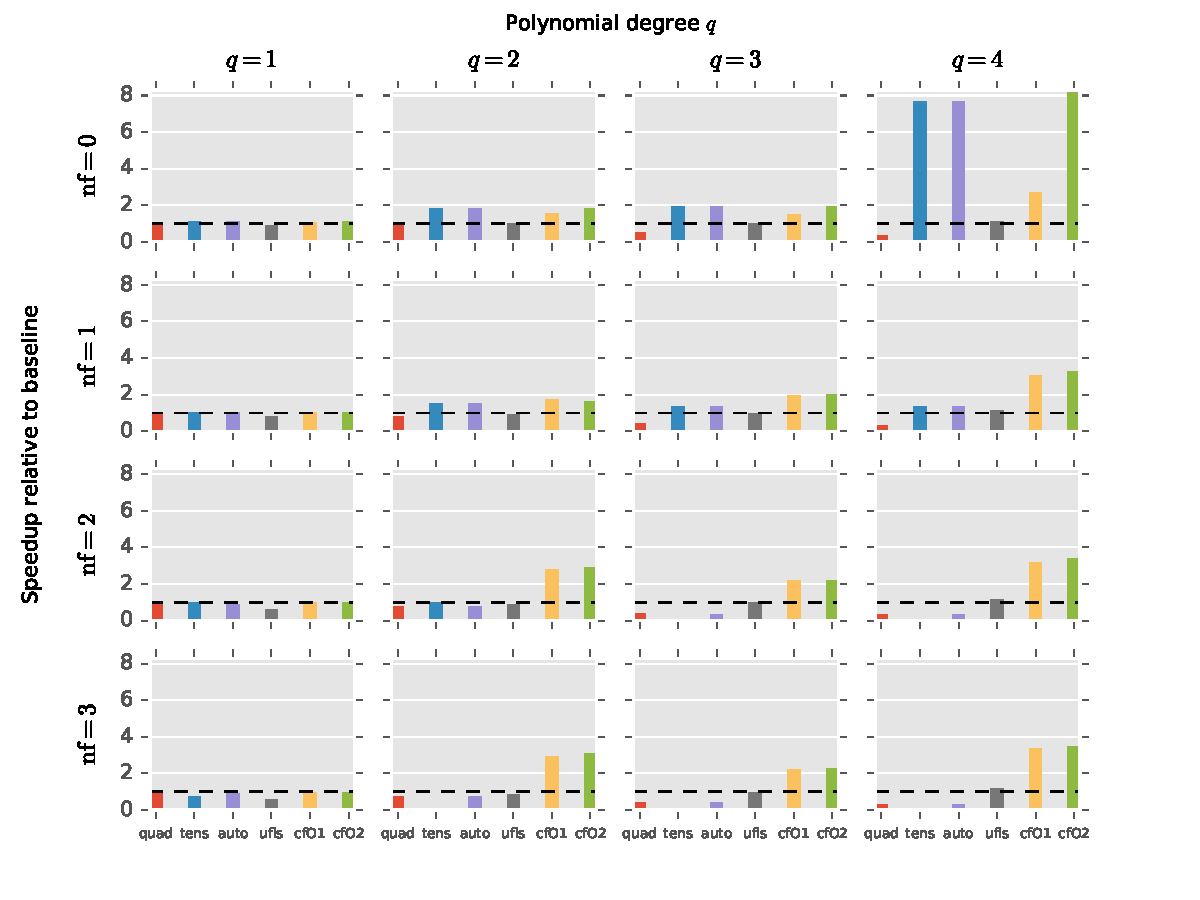
\includegraphics[scale=0.7]{perf-results/helmholtz}
\caption{Helmholtz results.}\label{fig:helmholtz}
\end{figure}
The results for the Helmholtz problem are provided in Figure~\ref{fig:helmholtz}. We observe that \texttt{ffc} slows the code down, especially for $q \geq 3$, as a consequence of using indirection arrays in the generated code that, as explained in Section~\ref{sec:zeros}, prevent, among the other compiler's optimizations, SIMD auto-vectorization. The \texttt{auto} version results in minimal performance improvements over \texttt{fix} when $nf=0$, unless $q=4$. This is due to the fact that if the loop over quadrature points is relatively small, then close-to-peak performance is obtainable through basic expression rewriting and code specialization; in this circumstance, generalized loop-invariant code motion and padding plus data alignment. The trend changes dramatically as $nf$ and $q$ increase: a more ample spectrum of transformations must be considered to find the optimal local assembly implementation. We will comment on this in details in the next section.

\paragraph{Elasticity}
\begin{figure}[t]  
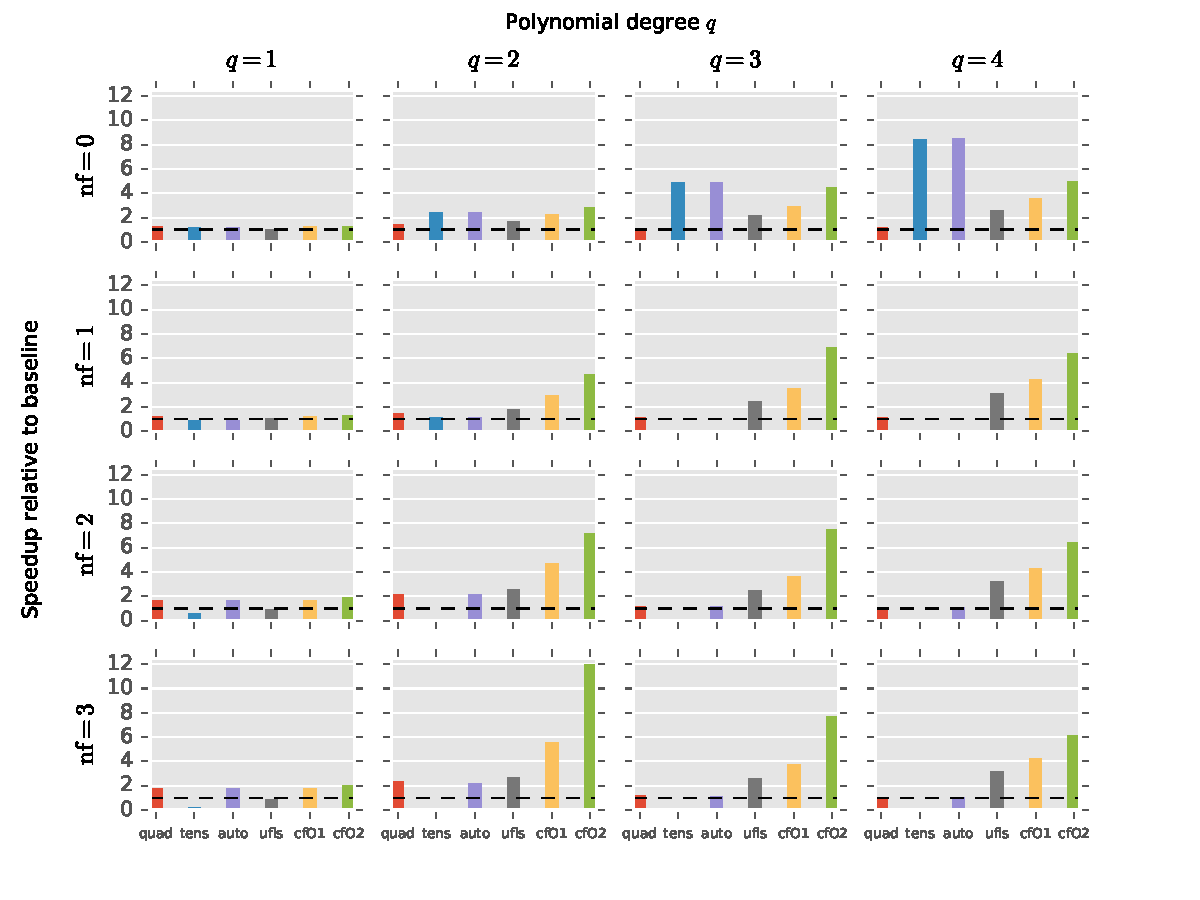
\includegraphics[scale=0.7]{perf-results/elasticity}
\caption{Elasticity results.}\label{fig:elasticity}
\end{figure}
Figure~\ref{fig:elasticity} illustrates results for the Elasticity problem. This form uses vector-valued spaces for the basis functions, so here transformations avoiding computation over zero-valued columns are of key importance. The \texttt{ffc} set of optimizations leads to notable improvements over the original code at $q=1$. The use of inderection arrays allows to phisically eliminate zero-valued columns at code generation time; as a consequence, different tabulated basis functions are merged into a single array. Therefore, despite the execution being purely scalar because of indirection arrays, the reduction in arithmetic intensity and register pressure imply improvement in performance. Nevertheless, \texttt{auto} remains in general the best choice, with gains over \texttt{ffc} that are wider as $p$ and $nf$ increase. 

For $q \geq 2$, in \texttt{ffc} the lack of SIMD vectorization counterbalances the decrease in the number of floating point operations, leading to speed ups over the original code that only occasionally exceeds 1$\times$. On the other hand, the successful application of the zero-avoidance optimization while preserving code specialization plays a key role for \texttt{auto}, resulting in much higher performance code especially at $q=2$ and $q=3$. 

It is worth noting that speed ups of \texttt{auto} over \texttt{fix} decrease at $q=4$, particularly for low values of $p$. As we will discuss in Section~\ref{sec:auto-analysis}, this is because at $q=4$ the vector-register tiling transformation (in combination with loop unroll-and-jam) leads to the highest performance. In principle, vector-register tiling can be used in combination to the zero-avoidance technique; however, due to mere technical limitations, this is currently not supported in COFFEE. Once solved, we expect much higher speed ups in the $q=4$ regime as well.

% TODO: mention aggressive expression rewriting somewhere

\paragraph{Poisson}
\begin{figure}[t]  
\includegraphics[scale=0.7]{perf-results/poisson}
\caption{Poisson results.}\label{fig:poisson}
\end{figure}

In Figure~\ref{fig:poisson} we report speed ups of \texttt{ffc}, \texttt{fix}, and \texttt{auto} over the original code for the Poisson form. We note that, as a general trend, \texttt{ffc} exhibits drops in performance as $nf$ increases, notably when $nf=3$, for any values of $q$ and $p$. This is a consequence of the inherent complexity of the generated code. The way \texttt{ffc} performs loop-invariant code motion leads to the pre-computation of integration-dependent terms at the level of the integration loop, which are characterized by higher arithmetic intensity and redundant computation as $nf$ increases. Moreover, the absence of vectorization is another limiting factor.

The \texttt{auto} variant generally shows the best performance. Significant improvements over \texttt{fix} are also achieved, notably as $q$, $p$ and $nf$ increase. As clarified in the next section, this is always due to a more aggressive expression rewriting in combination with the technique to avoid computation over the zero-valued columns induced by vector-valued function spaces.


\paragraph{Hyperelasticity}
\begin{figure}[t]  
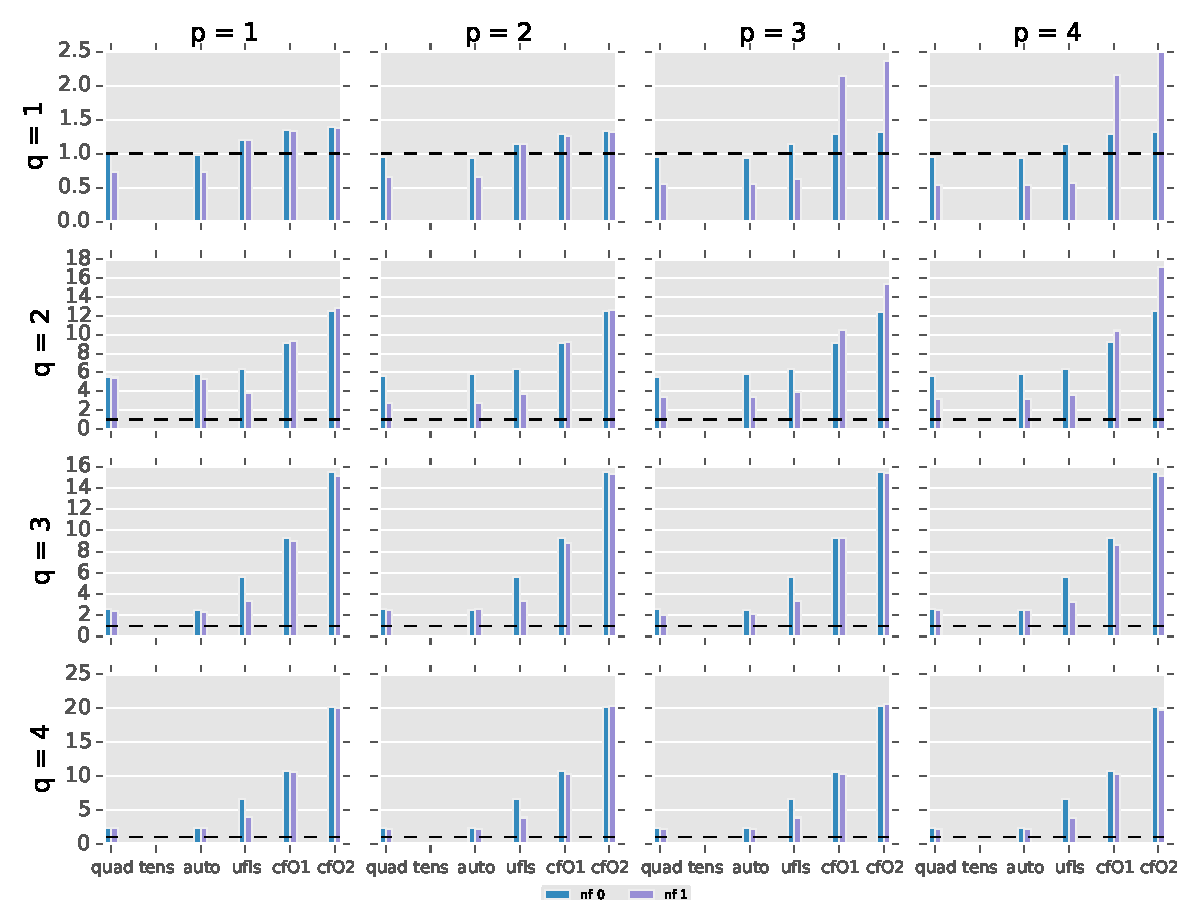
\includegraphics[scale=0.7]{perf-results/hyperelasticity}
\caption{Hyperelasticity results.}\label{fig:hyperelasticity}
\end{figure}

Speed ups for the hyperelasticity form are shown in Figure~\ref{fig:hyperelasticity}. Experiments for $nf \geq 3$ could not be executed because of FEniCS-Form-Compiler's technical limitations. 

For \texttt{auto}, massive speed ups for $q \geq 2$ must mainly be ascribed to aggressive and successful expression writing. Hyperelasticity problems are really compute-intensive, with thousands of operations being performed, so reductions in redundant and useless computation are crucial. Complex forms like hyperelasticity would benefit from further ``specialized'' optimizations: for example, it is a known technical limitation of COFFEE that, in some circumstances, less temporaries could (should) be generated and that hoisted code could (should) be suitably distributed over different loops to minimize register pressure (e.g. COFFEE could carefully apply loop fission for obtaining significantly better register usage). We expect to obtain considerably faster code once such optimizations will be incorporated. 

In the regime $q \geq 2$ and $nf=1$, peformance improvements are less pronounced moving from $p=1$ to $p=2$, although still significant; in particular, we notice a drop at $p=2$, followed by a raise up to $p=4$. It is worth observing that this effect is common to all set of optimizations. The hypothesis is that this is due to the way coefficient functions are evaluated at quadrature points (identical in all configurations), which cannot be easily vectorized unless a change in storage layout and loops order is implemented in the code (abstract syntax tree) generator on top of COFFEE. 


\subsection{Details on the Autotuning Process}
\label{sec:auto-analysis}

We first comment on the overhead of the autotuning process. In the context of Firedrake, the framework in which COFFEE is integrated, the autotuner is executed at run-time, once the local assembly kernels are provided by the FEniCS Form Compiler. Autotuning, therefore, introduces an overhead in the application execution time. For a given problem instance, such overhead originates from four sources: 1) creation of the various code variants; 2) generation of a C file containing such variants (as simple function calls, plus the ``main'' function that invokes the variants, in sequence); 3) compilation of the autotuning file; 4) execution. Of these four points, we note that: the cost of 4) is relatively small, because each variant's execution time is bound by an empirically-found value (e.g. some milliseconds). The cost of all four points is constrained by our heuristics to prune the search space, as described in Section~\ref{sec:autotune}. Moreover, for a given form and a given discretization, the autotuner needs to be executed only once, since its output is saved and reused for later assemblies. This implies that if the assembly occurs in a time stepping loop, or the same form is executed on a different mesh, or known quantities of the input problem are changed, then the assembly cost is rapidly amortized. Premised that, the most important thing remains that when working with real unstructured meshes - which are likely to be composed of millions of elements, leading to long-lasting assembly phases - the autotuner overhead practically becomes completely negligible. In our experience, and in particular in the four examined problems, the autotuning process lasted less than a minute in the majority of cases. Most often, it took less than thirty seconds. Rarely it needed more than a minute, specifically in the case of hyperelasticity; however, despite the inherent complexity of this form, we measured a peak of only 4 minutes for the extreme case $[q=4, p=4, nf=1]$, while 1.30 minutes were needed in the case $[q=1, p=1, nf=1]$. This analysis certifies that the autotuner overhead is definitely sustainable in real-world applications.

In this paper and in~\cite{Luporini}, we have repeatedly claimed that different forms (and different discretizations) require distinct sets of transformations to reach close-to-peak performance. To demonstrate this, we now report details about the output of the autotuning process. We show that for the four examined forms - more specifically, for the 224 problem instances $[form, q, p, nf]$ illustrated in the previous figures - a plethora of optimization strategies have been selected by the autotuner. We also complement and strengthen our claim by showing the autotuner's output for two additional forms whose performance results, for brevity, were not shown in Section~\ref{sec:perf-results-forms}: a Mass and a Mixed Poisson problems. 

Table~\ref{table:autotuner-output} shows the number a given transformation has been selected by the autotuner. To not hinder readability, the output has been grouped by form, rather than showing the selected optimization strategy for each $[form, q, p, nf]$. Values in the \texttt{rewrite strategy} column can either be \texttt{base} or \texttt{aggressive}, as explained in Section~\ref{sec:autotune}: in the former case, only generalized loop-invariant code motion in applied; in the latter case, the rewrite rules are recursively applied as extensive as possible. If the value of the column is \texttt{aggressive} (\texttt{base}) it means that in the majority of cases the \texttt{aggressive} (\texttt{base}) strategy prevailed on the \texttt{base} (\texttt{aggressive}) one. Precomputation of integration-dependent terms was explained in Section~\ref{sec:expr-rewriter-obj}. The \texttt{split} column refers to the expression splitting transformation (~\cite{Luporini}, and summary in Section~\ref{sec:summary-opts}). The \texttt{unroll} column indicates the application of explicit unrolling. Other columns are of obvious meaning. Values in the various columns illustrate the number of problem instances out of the total (column \texttt{mumber of variants}) in which an optimization was activated. Obviously, more transformations are typically used in combination in a same problem. 

%In the table, we implicitly assume that padding and data alignment (Section~\ref{sec:padding}), as well as precomputation of integration-dependent terms (Section~\ref{sec:expr-rewriter-obj}) have always been applied.



\newcommand{\autotuneroutput}{
\tiny
\begin{tabulary}{1.0\textwidth}{c|c|ccc|ccccc}
\cline{3-10}
\multicolumn{2}{c}{} & \multicolumn{3}{c|}{\texttt{expression rewriting}} & \multicolumn{5}{c}{\texttt{code specialization}} \\
\cline{1-10}
problem & \specialcell{number of\\variants} & \specialcell{rewrite\\strategy} & \specialcell{zero-valued columns\\avoidance} & \specialcell{precompute\\integration terms} & \specialcell{padding\\data alignment} & split & \specialcell{vector-register\\tiling} & unroll & BLAS \\
\cline{1-10}
\texttt{helmholtz} & 64 & aggressive & 0 & 0 & all & 8 & 17 & 15 & 0 \\
\texttt{mass} & 64 & base & 2 & 3 & 1 & 2 & 3 & 4 & 5 \\
\texttt{elasticity} & 64 & aggressive & 39 & 0 & all & 0 & 11 & 0 & 2 \\
\texttt{poisson} & 64 & aggressive & 50 & 0 & all & X & X & 1 & 0 \\
\texttt{mixed poisson} & X & base & 2 & 3 & 1 & 2 & 3 & 4 & 5 \\
\texttt{hyperelasticity} & 32 & aggressive & 2 & 3 & 1 & 2 & 3 & 4 & 5 \\
\cline{1-10}
\end{tabulary}
}

\begin{table*}[t]
\tbl{Autotuner output.}{ \scriptsize \autotuneroutput }
\label{table:autotuner-output}
\end{table*}

 
% selected variants (tables)
% show the difference of ``aggressive'' vs ``base'' expression rewriting

\section{Conclusions}
\label{sec:conclusions}

We have presented ...
...TODO...: straightforward extendibility to right-hand side assembly
% Mass DGEMM utile explicit method etc



% Bibliography
\bibliographystyle{ACM-Reference-Format-Journals}
\bibliography{biblio}


\medskip

\end{document}
